\ifdefined\pdfoutput\pdfoutput=1\fi % arXiv: compile with pdfLaTeX
\documentclass[11pt]{article}
\usepackage[margin=1in]{geometry}
\usepackage[T1]{fontenc}
\usepackage{lmodern}
\usepackage{microtype}
\usepackage{amsmath,amssymb,amsthm}
\usepackage{booktabs}
\usepackage{longtable}
\usepackage[skip=6pt]{caption}
\usepackage{graphicx}
\usepackage{xcolor}
\usepackage{listings}
\usepackage{enumitem}
\usepackage[hidelinks]{hyperref}
\usepackage[numbers,sort&compress]{natbib}

\newtheorem{proposition}{Proposition}
\newtheorem{definition}{Definition}
\lstset{basicstyle=\ttfamily\footnotesize,breaklines=true,frame=single,columns=fullflexible}
\setlist{itemsep=2pt,topsep=4pt}
\emergencystretch=3em

\newcommand{\HeadlineCount}{10}
\newcommand{\HeadlineMin}{0.52}
\newcommand{\HeadlineMax}{0.93}
\newcommand{\BookStart}{1 January 2019}
\newcommand{\BookHorizon}{31 December 2025}
\newcommand{\EarnedDriftPct}{at most 0.0004\%}
\newcommand{\IbnrErrRange}{-0.2\% to +2.2\%}
\newcommand{\BenchQuestions}{62}
\newcommand{\MaxTurns}{10}
\newcommand{\AccHaikuRaw}{77\%}
\newcommand{\AccHaikuDocs}{98\%}
\newcommand{\AccHaikuSemantic}{100\%}
\newcommand{\AccSonnetRaw}{84\%}
\newcommand{\AccSonnetDocs}{98\%}
\newcommand{\AccSonnetSemantic}{100\%}
\newcommand{\AdjRawHaiku}{98\%}
\newcommand{\ConvErrRawHaiku}{13}
\newcommand{\WrongRawHaiku}{14}
\newcommand{\GoldMentionedRawHaiku}{7}
\newcommand{\AdjRawSonnet}{98\%}
\newcommand{\ConvErrRawSonnet}{9}
\newcommand{\WrongRawSonnet}{10}
\newcommand{\GoldMentionedRawSonnet}{3}
\newcommand{\TestCount}{208}
\newcommand{\CrossChecks}{191}


\newcommand{\ResultsAbstract}{With raw tables, Claude Haiku~5.5 and Sonnet~5.5 answer \AccHaikuRaw{} and
\AccSonnetRaw{} of questions in line with the governed definitions. With the glossary they answer \AccHaikuDocs{},
and through the semantic layer they answer every question, at the lowest cost of the three conditions. Almost every
raw-schema error is an undiscoverable house convention, such as whether losses include ALAE or are net of
recoveries, rather than a reasoning failure: counted as correct, raw accuracy would be \AdjRawHaiku{}. The models
also found two defects in our own artefacts, which we report.}
\newcommand{\DiscussionGaps}{On ISL-Bench, almost all of the value sits in the first step: once the conventions are
written down, the models apply them nearly perfectly in SQL, and compiling them removes the residual day-count
slip and the one non-refusal. Executing the definitions buys consistency, refusals that come with a reason,
and roughly half the cost, rather than raw accuracy.}

\title{What Was the Loss Ratio?\\[4pt]
\large Time Basis and Valuation Date as First-Class Semantics in an Insurance Semantic Layer,\\
with a Benchmark for LLM Analytics}
\author{Hassan Raza\\ \small Independent researcher \quad \texttt{max@rfstudio.co}}
\date{\small Preprint, October 2026. Code and data: \url{https://github.com/maxraza/insurance-semantic-layer}}

\begin{document}
\maketitle

\begin{abstract}
In property and casualty insurance, a question as plain as ``what was the 2024 loss ratio?'' has many correct
answers. The answer depends on which date assigns a loss to the year (calendar, accident or policy year), which
loss measure is meant (paid, reported or ultimate, with or without loss adjustment expense), and the valuation
date at which the books are read. On a synthetic motor book we count \HeadlineCount{} defensible answers to that
question, ranging from \HeadlineMin{} to \HeadlineMax{}. Human analysts resolve this with conventions;
language models answering over raw tables resolve it silently. Current semantic-layer specifications do not
help, because they give a metric one time dimension and no valuation date. We make both explicit. We define
a small algebra of measure kinds (flow, earned, snapshot and valuation), each defined per time basis and
evaluated at a valuation date. We implement it as an open-source semantic layer that compiles to SQL and is
checked against an independent reference implementation. We also release ISL-Bench: \BenchQuestions{}
questions over a seeded synthetic UK personal-motor book with known ground truth, labelled for ambiguity and
answerability. We compare language models answering from raw schemas, from schemas with a business glossary,
and through the semantic layer as a tool. \ResultsAbstract{}
\end{abstract}

% ---------------------------------------------------------------------------------------------------------
\section{Introduction}

Ask an insurer's finance team, its reserving actuaries and its pricing team for last year's loss ratio and you
may get three different numbers, each correct. Finance reports the \emph{calendar-year} figure: claims paid in
the year plus the change in reserves, over premium earned in the year. Reserving looks at the \emph{accident
year}: losses on accidents that happened in the year, developed to the valuation date and grossed up for claims
not yet reported, over the same earned premium. Pricing often wants the \emph{policy} or underwriting year:
losses on policies written in the year, over the premium those policies earned. Each of these can be stated paid,
reported or ultimate, with or without allocated loss adjustment expense (ALAE), and each except the closed
calendar year changes every time the books are re-read. The textbooks are explicit that an aggregated loss
measure is not defined until the statistic, the aggregation method and the period, including its valuation
date, are fixed~\cite{werner2016basic,friedland2010estimating}.

This matters more now that language models answer questions over company data. A model given a schema and a
question will pick an interpretation, write SQL for it, and report a number, usually without saying which
interpretation it picked. Benchmarks for text-to-SQL score whether the query returns the gold result
set~\cite{yu2018spider,li2023bird,lei2025spider2}; they have no notion of a question with ten right answers, or
of a right answer that is ``this can't be computed from what we hold''. Semantic layers, which put governed
metric definitions between the user and the tables, are the usual remedy, and there is growing evidence that
they improve LLM accuracy on enterprise data~\cite{sequeda2023benchmark,allemang2024ontologies,ganz2026sltext2sql}.
But the specifications they are built on (MetricFlow, Cube, LookML, and the new Open Semantic Interchange
draft) model a metric as an aggregate over a table with a single time dimension~\cite{dbt_metrics_docs,
cube_measures_docs,lookml_docs,osi_spec}. They cannot say ``this measure means something different on an
accident basis'', or ``use only what was known at 31 December''.

\paragraph{Contributions.}
\begin{enumerate}
\item A model of insurance metrics in which a measure is defined \emph{per time basis}, and every query must
name a basis and a valuation date (Section~\ref{sec:model}). Four measure kinds (flow, earned, snapshot and
valuation) cover written and earned premium, exposure, paid and reported losses, case reserves, booked IBNR,
claim counts, expenses, quotes and renewals. Ratios are always ratios of sums. A dimension is only usable if
every measure in a metric supports it, and a basis is only usable if every measure is defined on it, so
undefined questions are rejected rather than answered.
\item An open-source implementation: a YAML semantic model, a compiler to readable DuckDB SQL, and an independent
reference implementation in plain Python. The two are cross-checked on every measure and basis, and the cross-check
catches deliberately injected semantic bugs (Section~\ref{sec:impl}).
\item A seeded synthetic UK personal-motor book, generated forward in time with real-world mess: price-comparison
quoting, mid-term changes, cancellations, renewal pricing under a regulatory cap, late-reported claims, case
reserving, recoveries, and quarterly chain-ladder IBNR. Facts after the data horizon are withheld from the
published tables, and the final cost of every accident is kept as ground truth (Section~\ref{sec:book}).
\item ISL-Bench, a benchmark of \BenchQuestions{} questions with gold answers computed by the semantic layer,
labelled traps for common misreadings, ambiguous questions with every defensible answer enumerated, and
unanswerable questions. We report results for current Claude models under three conditions
(Sections~\ref{sec:bench}--\ref{sec:results}).
\end{enumerate}

Everything in this paper is synthetic and reproducible from a seed. No real policyholder, insurer or employer
data was used.

% ---------------------------------------------------------------------------------------------------------
\section{Background and related work}\label{sec:background}

\paragraph{Insurance metrics.}
Werner and Modlin define written premium as the premium on policies issued in a period, earned premium as the
portion of written premium for which coverage has already been provided, and the loss ratio as losses over
premium, ``typically'' reported losses over earned premium~\cite[pp.~2--9]{werner2016basic}. Every aggregated
loss measure is fixed by a statistic (paid or reported), an aggregation method (calendar, accident, policy or
report year), and a period consisting of an accounting period and a valuation
date~\cite[p.~91]{werner2016basic}. Friedland separates the accounting date (which claims are in scope) from the
valuation date (which transactions are included), and avoids the word ``incurred'' because readers cannot tell
whether it includes IBNR~\cite[pp.~15, 38--39]{friedland2010estimating}. Calendar-year figures are fixed once
the year closes; accident- and policy-year figures develop until every claim
settles~\cite[pp.~42--43]{werner2016basic}. The conventional accident-year loss ratio pairs accident-year losses
with calendar-year earned premium, and the policy-year ratio pairs both sides by inception
date~\cite[p.~43]{werner2016basic}. US statutory Schedule~P now groups losses by ``incurred year'', the year
of whatever event triggers coverage~\cite{naic2025bwg07}. The OMG Property~\& Casualty Data Model gives the
entities (policy, policy coverage detail, claim, claim amount, policy amount with earning begin and end dates) on
which such data is usually held~\cite{omg2014pc}. For UK motor, renewal prices have been capped at the equivalent
new-business price since 2022, and each price-comparison site counts as a separate distribution
channel~\cite{fca2021ps215}.

\paragraph{Semantic layers.}
Dimensional modelling distinguishes additive facts, semi-additive facts (balances, which add across every
dimension except time) and non-additive facts such as ratios, which should be computed from summed components
at the end~\cite{kimball_additive,kimball2013toolkit}. MetricFlow, the engine behind the dbt Semantic Layer,
has simple, ratio, cumulative, derived and conversion metrics, a default aggregation time dimension per model,
and semi-additive measures through \texttt{non\_additive\_dimension}~\cite{dbt_metrics_docs,dbt_measures_docs}.
It also restricts joins to avoid fan-out~\cite{dbt_joins_docs}. Cube, LookML and Malloy each handle fan-out in
their own way: Cube with deduplication, LookML with symmetric aggregates and Malloy with aggregate
locality~\cite{cube_joins_docs,looker_symmetric_docs,malloy_aggregates_docs}. The Open Semantic Interchange
draft (now Apache Ossie) defines datasets, fields, relationships and metrics, with an \texttt{ai\_context} for
instructions and synonyms, but no additivity, time-grain or ratio construct~\cite{osi_spec,osi_launch_2025}. None
of these systems lets a measure's \emph{definition} depend on a time basis chosen at query time, and none has a
valuation date.

\paragraph{LLMs over enterprise data.}
Text-to-SQL accuracy that looks high on Spider and BIRD falls sharply on enterprise
schemas~\cite{yu2018spider,li2023bird}. The same agent scores 91.2\% on Spider~1.0 and 17--21\% on
Spider~2.0~\cite{lei2025spider2}, and the best system on BEAVER scores about 11\%~\cite{chen2024beaver}.
Error taxonomies for LLM-generated SQL have no category for using the wrong metric
definition~\cite{liu2025nl2sqlbugs,shen2026icl}. The closest prior work is Sequeda, Allemang and Jacob's
benchmark on a 13-table subset of the OMG P\&C model. In it, GPT-4 answered 16.7\% of 43 questions correctly
from SQL and 54.2\% with a knowledge graph~\cite{sequeda2023benchmark,sequeda2024benchmark_grades}. A follow-up
reached 72.6\% with ontology-based query checking and repair~\cite{allemang2024ontologies}. Practitioner
replications with the dbt Semantic Layer report similar gains, and note that the semantic layer declines
questions it cannot express rather than answering them wrongly~\cite{ganz2023semanticlayer,ganz2026sltext2sql}.
Recent preprints compile LLM output in a constrained intermediate representation into SQL, with large
improvements~\cite{ai2026spc,kim2026smq,pillai2026ground,rumiantsau2026semantic,ye2026contextlayer}. Insurance-specific
LLM work has addressed actuarial reasoning and question answering rather than governed
KPIs~\cite{balona2024actuarygpt,hao2025reinsurance,chen2026insactbench,ding2025insqabench}. AMBROSIA studies
ambiguous questions in text-to-SQL~\cite{saparina2024ambrosia}; we add the domain case where the ambiguity is
a choice of convention, and the case where the right answer is a refusal.

% ---------------------------------------------------------------------------------------------------------
\section{A model of insurance metrics}\label{sec:model}

\paragraph{Facts.}
A \emph{fact} $f$ has an amount $a_f$, a set of dimension values, a \emph{knowledge date} $k_f$ (when the insurer
learned of it: the booking, report, transaction or valuation date), and one or more \emph{business dates}. These
are the dates a basis can use to assign the fact to a period: transaction date, accident date, or the inception
date of the covering policy term. Premium facts also carry a cover interval $[s_f, e_f)$.

\paragraph{Queries.}
A query is $Q = (M, \beta, \tau, g, D, F)$: metrics $M$, a time basis $\beta \in
\{\textsc{cal}, \textsc{acc}, \textsc{pol}\}$, a valuation date $\tau$, a grain $g$ (year, quarter, month) that
partitions time into periods $p = [p^-, p^+)$, group-by dimensions $D$ and filters $F$. Both $\beta$ and $\tau$
are mandatory. A measure $\mu$ is a partial map from bases to definitions; $\mu(\beta)$ may be undefined.

\begin{definition}[Measure kinds]
Let $d_\beta(f)$ be the business date basis $\beta$ uses for fact $f$, and $\mathcal{K}_\tau = \{f : k_f \le
\tau\}$ the facts known at $\tau$. For a period $p$ with $p^- \le \tau$:
\begin{align*}
\textbf{flow:}\quad & \mu_\beta(p,\tau) = \textstyle\sum_{f \in \mathcal{K}_\tau,\; d_\beta(f) \in p} a_f \\
\textbf{earned:}\quad & \mu_\beta(p,\tau) = \textstyle\sum_{f \in \mathcal{K}_\tau} a_f \,
  \dfrac{\big|[s_f, e_f) \cap p \cap (-\infty, \tau]\big|}{|[s_f, e_f)|}
  \quad (\beta \in \{\textsc{cal},\textsc{acc}\}) \\
& \mu_{\textsc{pol}}(p,\tau) = \textstyle\sum_{f \in \mathcal{K}_\tau,\; d_{\textsc{pol}}(f) \in p} a_f \,
  \dfrac{\big|[s_f, e_f) \cap (-\infty, \tau]\big|}{|[s_f, e_f)|} \\
\textbf{snapshot:}\quad & \mu(p,\tau) = \textstyle\sum_{f \in \mathcal{K}_{t},\; \phi(f, t)} a_f(t),
  \qquad t = \min(p^+ - 1, \tau) \\
\textbf{valuation:}\quad & \mu_{\textsc{acc}}(y,\tau) = V(v^*_\tau, y), \qquad v^*_t = \max\{v : v \le t\} \\
& \mu_{\textsc{cal}}(p,\tau) = \textstyle\sum_y V(v^*_{t}, y) - \sum_y V(v^*_{p^- - 1}, y)
\end{align*}
where $\phi$ is a membership condition (in force at $t$, open at $t$), $a_f(t)$ may depend on $t$ (unearned
premium), and $V(v, y)$ is the estimate booked at valuation $v$ for cohort $y$ (IBNR by accident year).
\end{definition}

Metrics are arithmetic over measures, evaluated per output cell after aggregation:
$\mathrm{LR}^{\mathrm{rep}}_\beta(p,\tau) = \mathrm{RL}_\beta(p,\tau) / \mathrm{EP}_\beta(p,\tau)$, never as an
average of finer-grained ratios. The accident-basis earned premium equals the calendar one, which encodes the
standard pairing of accident-year losses with calendar-year earned premium. A metric is defined on $\beta$ only
if all of its measures are, and can be grouped or filtered by a dimension only if all of its measures carry it
(\emph{conformance}). In the motor model, IBNR is booked by accident year only, so the ultimate loss ratio has
no policy basis and cannot be split by channel. Premium has no peril, so no loss ratio can be split by peril.

\begin{proposition}[Calendar flows close]
If $d_{\textsc{cal}}(f) = k_f$ for every fact (as for claim transactions), then
$\mu_{\textsc{cal}}(p,\tau) = \mu_{\textsc{cal}}(p,\tau')$ for all $\tau, \tau' \ge p^+ - 1$.
\end{proposition}
\begin{proof}
Every fact with $d_{\textsc{cal}}(f) \in p$ has $k_f < p^+ \le \tau$, so it is in both $\mathcal{K}_\tau$ and
$\mathcal{K}_{\tau'}$.
\end{proof}
Accident and policy flows have no such property: a fact with business date in $p$ can have any later knowledge
date, which is exactly loss development. Calendar \emph{earned} premium closes only if no premium transaction is
booked after its effective date. Back-dated cancellations and mid-term adjustments break that, and on our book
the closed-year earned premium moves by \EarnedDriftPct{} after close.

\begin{proposition}[Ratios of sums]
For periods $p_1,\dots,p_n$ partitioning $p$, $\frac{\sum_i L_i}{\sum_i E_i} = \sum_i w_i \frac{L_i}{E_i}$ with
$w_i = E_i / \sum_j E_j$, so the mean of sub-period ratios equals the period ratio only when all $E_i$ are equal.
\end{proposition}
The weights are the earned-premium shares, so with seasonal or growing premium the unweighted mean of quarterly
loss ratios is biased toward the low-premium quarters. ISL-Bench includes this trap (Section~\ref{sec:bench}).

\begin{proposition}[Earning integrates to written]
For the \textsc{pol} basis and $\tau \ge \max_f e_f$, earned premium equals written premium for every cohort.
\end{proposition}
\begin{proof}
Each fact contributes $a_f \cdot |[s_f,e_f)| / |[s_f,e_f)| = a_f$.
\end{proof}

% ---------------------------------------------------------------------------------------------------------
\section{Implementation}\label{sec:impl}

The semantic model is a YAML file (Appendix~\ref{app:model}). It declares \emph{sources} (a FROM clause, a
knowledge-date column and the dimensions available on it), \emph{measures} (a source, an amount or count, an
optional filter, and one definition per supported basis), and \emph{metrics} (arithmetic expressions over
measures). The compiler knows the four kinds and nothing about insurance. It validates the query, emits one
common table expression per measure over a generated period grid, joins the measures on period and group-by
keys, and computes metric expressions with null-safe division. The output is plain DuckDB SQL a reviewer can
read; Appendix~\ref{app:sql} shows the SQL for an accident-year ultimate loss ratio. Snapshot measures join the
period grid on a condition evaluated at $\min(p^+ - 1, \tau)$, and valuation measures use an \texttt{ASOF} join
to pick the latest booked estimate.

\paragraph{Differential testing.}
A second implementation computes every measure directly from the raw rows in Python, with no SQL and no code
shared with the compiler. The test suite compares the two on every measure and metric under every basis it
allows, at mid-period valuation dates (so that as-of clipping matters), plus 60 random queries with group-by and
filters: \CrossChecks{} comparisons in all. Two mutation checks confirm the comparison has teeth. Dropping the
valuation-date clip from earning, and snapshotting case reserves at $\tau$ instead of the period end, are each
caught. Further tests cover the specification's scenarios: a mid-year policy earns 368 of 730 in its first
calendar year, valuation dates hide later facts, yearly ratios are not means of quarterly ones, and
non-conformed dimensions are rejected.

% ---------------------------------------------------------------------------------------------------------
\section{A synthetic motor book}\label{sec:book}

The generator simulates a direct UK motor insurer from \BookStart{} to a data horizon of \BookHorizon{}, forward
in time. Quotes arrive monthly with January seasonality and growth. About two-thirds come through
price-comparison sites, where our price is ranked against nine competitors and conversion falls with rank. Bound
quotes become annual terms. Terms can have a mid-term adjustment, a pro-rata cancellation, and a renewal
invitation three weeks before expiry. The renewal price is the equivalent new-business price for the same risk
and claims history, with a tenure margin before 2022 and capped at that price afterwards~\cite{fca2021ps215}.
Acceptance depends on the price change and channel. Claims arrive by peril as Poisson processes over covered
days, with risk relativities by region, vehicle group, driver age and no-claims years. Each claim is reported
after a peril-specific delay (bodily injury is slow), reserved, partly paid, re-reserved, paid, and closed;
some are nil, and some own-damage and third-party claims have later recoveries. Claims inflation peaks in
2022--23, ahead of rate increases. At every quarter-end, IBNR is booked by accident year from a volume-weighted
chain ladder on the accident-quarter by development-quarter incurred triangle, using only data known on that
date. Facts dated after the horizon are dropped from the published tables. The final cost of every accident up
to the horizon, reported or not, is kept in a ground-truth table that is never shown to a model.

\begin{table}[t]\centering\small
\caption{The synthetic book (seed 7, horizon 31 December 2025).}\label{tab:book}
\begin{tabular}{lr}\toprule
Quotes & 892,296 \\
Policy terms (incl.\ renewals) & 210,319 \\
Premium transactions & 245,710 \\
Claims reported & 23,549 \\
Claim transactions & 120,247 \\
Quarterly IBNR valuations & 25 \\
Written premium 2025 (GBP m) & 30.3 \\
Vehicles in force at horizon & 39,920 \\
PCW share of quotes & 68\% \\
Renewal retention 2025 & 68.9\% \\
Claim frequency AY2024 (per car-year) & 0.133 \\
\bottomrule\end{tabular}\end{table}


Table~\ref{tab:book} summarises the book. Because the truth is known, the booked estimates can be checked: at
the horizon, reported loss plus booked IBNR is within \IbnrErrRange{} of the true ultimate for every accident
year. Accounting invariants are tested: reports follow accidents within cover; case reserves never go negative
and are zero on closed claims; nothing is known after the horizon; renewal prices respect the cap; and expired
cohorts earn exactly their written premium.

% ---------------------------------------------------------------------------------------------------------
\section{ISL-Bench}\label{sec:bench}

\paragraph{Questions.}
ISL-Bench has \BenchQuestions{} questions in ten categories (Table~\ref{tab:categories}). \emph{Control}
questions have no hidden semantics, such as how many quotes were issued in 2024. Then come \emph{earning},
\emph{time basis}, \emph{valuation} date, \emph{loss definition}, ratio \emph{aggregation}, \emph{snapshot}
balances, \emph{counting} conventions and \emph{retention}. \emph{Ambiguous} questions (``what was our loss ratio
in 2024?'') accept every defensible interpretation. \emph{Unanswerable} questions (a loss ratio by peril, a
booked policy-year ultimate, a channel-level ultimate, a forecast) are correct only if declined. Every answer is
a single number. Gold values are computed by the semantic layer from declarative cells (metric, basis, period,
valuation date, filters, and a reduction over periods), so the questions file is readable and auditable. Most
questions also list \emph{traps}: plausible misreadings such as calendar instead of accident year, written
instead of earned, or the current valuation instead of the stated one. A wrong answer that matches a trap is
labelled with it.

\paragraph{Conditions.}
All conditions share the same instructions: the data runs to 31 December 2025, values are as at that date unless
stated, use the tools, say so if the question cannot be answered, and end with a single \texttt{ANSWER:} line.
\begin{itemize}
\item \textbf{Raw}: the schema DDL without comments, and a read-only SQL tool over a copy of the book without the
truth table.
\item \textbf{Docs}: the commented DDL plus a business glossary that renders the semantic model as prose, with
the time-basis and valuation conventions, every measure's definition, bases and dimensions, and every metric's
formula, plus the same SQL tool. This isolates the effect of \emph{knowing} the definitions from the effect of
\emph{having them compiled}.
\item \textbf{Semantic}: no SQL. The only tool is \texttt{query\_metrics}, whose JSON schema enumerates the
metrics, bases and dimensions, and whose errors are the compiler's rejection messages.
\end{itemize}
Each question runs as an agentic loop of up to \MaxTurns{} turns. Current Claude models do not accept a
sampling temperature, so we run each question once per condition and cache every response. The tables can be
regenerated from the cache without API calls.

\paragraph{Scoring.}
An answer is correct if it is within 0.2\% of the gold value or of any accepted interpretation. Ratios get an
absolute tolerance of 0.0006 to allow three-decimal rounding, and are also accepted as percentages. For ambiguous
questions we also record \emph{disclosure}: whether the explanation names a time basis or a loss or premium
definition. This uses a fixed regular expression, which over-counts rather than under-counts.

% ---------------------------------------------------------------------------------------------------------
\section{Results}\label{sec:results}

\begin{figure}[t]\centering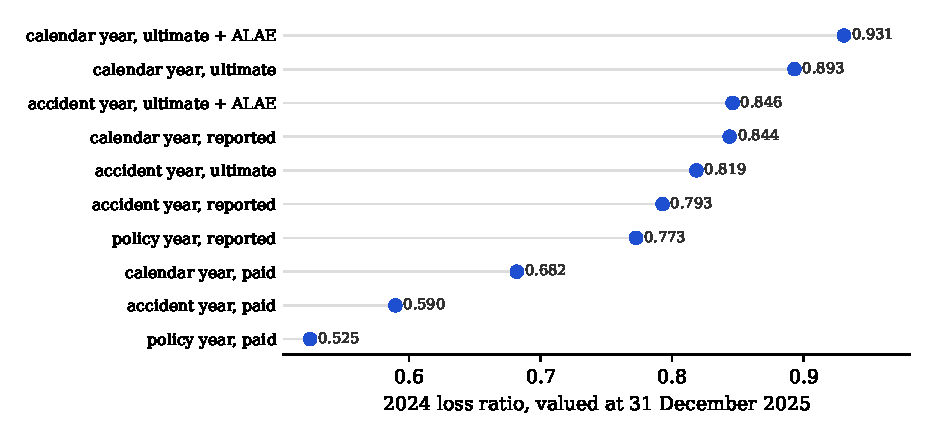
\includegraphics[width=\linewidth]{figures/answers.pdf}
\caption{Every defensible answer to ``what was the 2024 loss ratio?'' on the synthetic book, valued at 31
December 2025, as computed by the semantic layer. Ultimate figures include booked IBNR; the policy-year basis
has no booked IBNR, so no policy-year ultimate exists.}\label{fig:answers}\end{figure}

\begin{figure}[t]\centering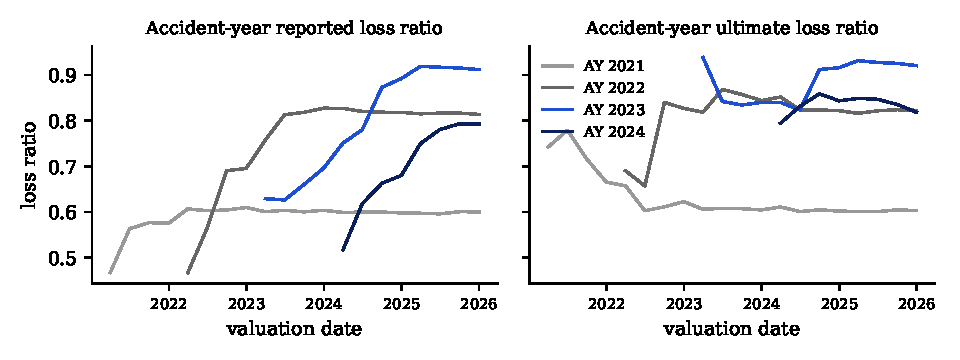
\includegraphics[width=\linewidth]{figures/development.pdf}
\caption{The same accident year read at successive quarter-end valuation dates. Reported loss ratios rise as
late claims are reported and reserves develop; adding booked IBNR anticipates much of that development.}
\label{fig:development}\end{figure}

\begin{table}[t]\centering\small
\caption{ISL-Bench results. Accuracy over all questions with a 95\% bootstrap interval over questions; accuracy on the answerable, unambiguous core; ambiguous questions answered with a defensible value (and, in brackets, how many answers named a basis or definition); unanswerable questions declined; wrong answers (in brackets, how many quoted the governed figure in their explanation); API cost.}\label{tab:main}
\resizebox{\linewidth}{!}{\begin{tabular}{llrrrrrr}\toprule
Model & Condition & All & Core & Ambiguous (disclosed) & Unanswerable & Wrong (quoted) & Cost \\ \midrule
Haiku 5.5 & raw & 77\% [66\%, 87\%] & 73\% & 7/7 (7) & 4/4 & 14 (7) & \$0.13 \\
Haiku 5.5 & docs & 98\% [95\%, 100\%] & 98\% & 7/7 (7) & 4/4 & 1 (1) & \$0.07 \\
Haiku 5.5 & semantic & 100\% [100\%, 100\%] & 100\% & 7/7 (7) & 4/4 & 0 (0) & \$0.02 \\
Sonnet 5.5 & raw & 84\% [74\%, 94\%] & 82\% & 7/7 (7) & 3/4 & 10 (3) & \$0.88 \\
Sonnet 5.5 & docs & 98\% [95\%, 100\%] & 100\% & 7/7 (7) & 3/4 & 1 (0) & \$0.58 \\
Sonnet 5.5 & semantic & 100\% [100\%, 100\%] & 100\% & 7/7 (7) & 4/4 & 0 (0) & \$0.39 \\
\bottomrule\end{tabular}}\end{table}

\begin{table}[t]\centering\small
\caption{Correct answers by question category (number of questions in brackets).}\label{tab:categories}
\resizebox{\linewidth}{!}{\begin{tabular}{lrrrrrr}\toprule
Category & Haiku raw & Haiku doc & Haiku sem & Sonnet raw & Sonnet doc & Sonnet sem \\ \midrule
Control (7) & 7/7 & 7/7 & 7/7 & 7/7 & 7/7 & 7/7 \\
Earning (6) & 5/6 & 5/6 & 6/6 & 6/6 & 6/6 & 6/6 \\
Time basis (8) & 3/8 & 8/8 & 8/8 & 5/8 & 8/8 & 8/8 \\
Valuation (5) & 2/5 & 5/5 & 5/5 & 2/5 & 5/5 & 5/5 \\
Loss definition (7) & 5/7 & 7/7 & 7/7 & 7/7 & 7/7 & 7/7 \\
Aggregation (7) & 4/7 & 7/7 & 7/7 & 4/7 & 7/7 & 7/7 \\
Snapshot (5) & 5/5 & 5/5 & 5/5 & 5/5 & 5/5 & 5/5 \\
Counting (2) & 2/2 & 2/2 & 2/2 & 2/2 & 2/2 & 2/2 \\
Retention (4) & 4/4 & 4/4 & 4/4 & 4/4 & 4/4 & 4/4 \\
Ambiguous (7) & 7/7 & 7/7 & 7/7 & 7/7 & 7/7 & 7/7 \\
Unanswerable (4) & 4/4 & 4/4 & 4/4 & 3/4 & 3/4 & 4/4 \\
\midrule Mean tool calls & 4.5 & 2.2 & 1.1 & 2.8 & 1.1 & 1.0 \\
\bottomrule\end{tabular}}\end{table}

\begin{table}[t]\centering\small
\caption{Every incorrect answer, classified from the model's own explanation. The first three classes are house conventions that cannot be discovered from raw tables.}\label{tab:errors}
\resizebox{\linewidth}{!}{\begin{tabular}{lrrrrrr}\toprule
Error class & Haiku raw & Haiku doc & Haiku sem & Sonnet raw & Sonnet doc & Sonnet sem \\ \midrule
ALAE included in losses & 9 & 0 & 0 & 7 & 0 & 0 \\
Recoveries not netted & 2 & 0 & 0 & 2 & 0 & 0 \\
Day-count convention & 2 & 1 & 0 & 0 & 0 & 0 \\
Wrong cohort definition & 1 & 0 & 0 & 0 & 0 & 0 \\
Answered a different question & 0 & 0 & 0 & 0 & 1 & 0 \\
Estimated instead of declining & 0 & 0 & 0 & 1 & 0 & 0 \\
\bottomrule\end{tabular}}\end{table}

% Hand-written narrative for Section 7. Every number is a macro from generated/numbers.tex
% or a cell in the generated tables, so it moves with the data.

\paragraph{One question, many answers.}
Figure~\ref{fig:answers} shows the problem the paper starts from: \HeadlineCount{} defensible values for the
2024 loss ratio, from \HeadlineMin{} (policy year, paid) to \HeadlineMax{} (calendar year, ultimate including
ALAE). None of them is an error. Figure~\ref{fig:development} shows why the valuation date has to be part of
the question. The reported loss ratio for accident years 2022--2024, read at their own year end and again at the horizon,
rises by 11 to 22 points as late claims arrive and reserves develop. Booked IBNR anticipates most of that
movement: the ultimate ratio moves by under three points for 2022 and 2024, but by eight points for 2023, the
year in which claims inflation outran the development pattern the chain ladder had learned.

\paragraph{Accuracy.}
Table~\ref{tab:main} reports accuracy against the governed definitions. With raw tables, Haiku~5.5 answers
\AccHaikuRaw{} of questions correctly and Sonnet~5.5 \AccSonnetRaw{}. With the glossary both reach
\AccHaikuDocs{}, and through the semantic layer both answer every question correctly. Every condition handled
the ambiguous questions with a defensible value and named its interpretation. Every condition except
Sonnet's two SQL conditions declined all four unanswerable questions (below).

\paragraph{What the raw-schema errors are.}
Table~\ref{tab:errors} classifies every wrong answer from the model's own explanation. The striking result is
how few of them are reasoning errors. No model confused calendar with accident year, used written for earned
premium, ignored a stated valuation date, averaged quarterly ratios, or summed a balance across periods. Those
are the misreadings the benchmark's traps were designed to catch, and none was triggered. \ConvErrRawHaiku{} of Haiku's
\WrongRawHaiku{} raw-schema errors, and \ConvErrRawSonnet{} of Sonnet's \WrongRawSonnet{}, are \emph{house
conventions} that no schema reveals. The three conventions are:
\begin{itemize}
\item whether ``reported'' or ``incurred'' losses include ALAE, which the models mostly included and the house
definition excludes;
\item whether paid losses are net of subrogation and salvage recoveries;
\item whether the valuation day itself is earned.
\end{itemize}
The models usually said which choice they made, and in \GoldMentionedRawHaiku{} (Haiku) and
\GoldMentionedRawSonnet{} (Sonnet) cases they quoted the governed figure as the alternative. Counting those
convention choices as correct, raw-schema accuracy would be \AdjRawHaiku{} for Haiku and \AdjRawSonnet{} for
Sonnet. On this benchmark, then, a current model with database access and no documentation gets the
\emph{reasoning} right and the \emph{conventions} wrong. The one genuine reasoning error is Haiku building a
policy-year cohort from each policy's first inception date rather than each term's.

\paragraph{Refusals.}
Sonnet with raw tables answered one unanswerable question, the booked policy-year ultimate loss ratio. It
allocated accident-year IBNR to policy years in proportion to incurred losses and said so. That is a reasonable
actuarial estimate, but not a booked figure, and the governed layer declines it. Sonnet with the glossary
answered ``loss ratio for windscreen claims'' with windscreen's contribution to the total loss ratio, and said
that too. Through the semantic layer, both models declined all four, and the refusal text was the compiler's
reason (premium is not split by peril; IBNR is booked by accident year and not allocated to channels).

\paragraph{Cost and effort.}
The semantic layer is also the cheapest condition (Table~\ref{tab:main}). Sonnet's whole run cost
\$0.39 through the semantic layer against \$0.88 with raw tables, and it needed far fewer tool calls
(Table~\ref{tab:categories}). Raw-schema runs spend most of their calls profiling tables and reconciling
movements before they compute anything.

\paragraph{What the benchmark found in the benchmark.}
Two findings were about our own artefacts, and we report them because they illustrate the paper's argument.
First, in the pilot both models' raw-SQL answers for earned exposure disagreed with our gold value by 3.5\%. The
models were right: the generator booked a full car-year of negative exposure on cancellation instead of the
unexpired fraction. We fixed the generator, added a regression test that reconciles earned exposure with
covered days, and re-ran the affected questions. Second, Sonnet with raw tables declined the 2025 expense ratio.
Its reason was that December's expenses are booked in January, so at 31 December 2025 the year is incomplete.
The semantic layer had happily divided eleven months of expenses by twelve months of premium. Valuation dates
make incompleteness \emph{visible} in the data, but our layer does not yet \emph{flag} it (Section~\ref{sec:discussion}).
We moved the two expense questions to 2024, and added to one ambiguous question (``incurred losses'') the
readings that include ALAE. All changes were made after the pilot and are marked in the questions file.



% ---------------------------------------------------------------------------------------------------------
\section{Discussion}\label{sec:discussion}

\paragraph{What the semantic layer contributes.}
The docs condition gives the model the same definitions as the semantic layer, in prose. The gap between docs
and semantic is therefore the value of having definitions \emph{executed} rather than \emph{described}: earning
arithmetic, valuation clipping, snapshot timing and ratio-of-sums that the model no longer has to get right in SQL.
The gap between raw and docs is the value of writing the conventions down at all. \DiscussionGaps{}

\paragraph{Refusal is a feature.}
A semantic layer that refuses a loss ratio by peril is doing the analyst a service: there is no peril-level
premium, and any number would rest on an allocation nobody chose. In our model, refusals come from two
structural checks, basis-definedness and dimensional conformance. Both are cheap to implement and both are absent
from current interchange specifications.

\paragraph{Completeness is part of valuation.}
A valuation date tells the layer which facts to use. It does not tell the layer whether a period is complete
at that date. Our layer returned a 2025 expense ratio at 31 December 2025 built on eleven months of expenses,
and a model with raw tables noticed. The fix is a third piece of metadata per source: the delay after which a
period's facts are expected to be complete (here, expense booking lag), so the compiler can flag or refuse
cells valued before then. Accident-year losses are never complete in this sense, which is what IBNR is for.
Expenses and premium are complete within days, and saying so is cheap.

\paragraph{A proposal for interchange formats.}
The Open Semantic Interchange draft has an \texttt{ai\_context} block but no way to say that a measure is
semi-additive, that a metric is a ratio of sums, or that a measure's definition varies with the time basis. We
suggest three additions, all expressible in the YAML of Appendix~\ref{app:model}. First, a per-measure map from
time basis to definition. Second, a mandatory query-time valuation date, applied through a declared knowledge
date on every source. Third, a measure kind (flow, earned over an interval, snapshot, or booked valuation)
from which additivity follows.

% ---------------------------------------------------------------------------------------------------------
\section{Limitations}\label{sec:limits}

The book is synthetic. It is calibrated for plausibility, not fitted to any market, and real data is messier:
backdated corrections, reopened claims, reinsurance and multiple currencies. The benchmark was written by the
author of the method it evaluates. We mitigate this by publishing every question, gold cell, trap, prompt and
raw response, and by including control questions on which the semantic layer should not help. We evaluate two
models from one family, with one run per question, so differences of a few questions are within noise; confidence
intervals in Table~\ref{tab:main} are bootstrap intervals over questions. Gold values come from the semantic
layer itself, so the semantic condition is partly a test of whether the model chose the right parameters; the
docs condition, which has no compiler, is the fairer comparison for the value of definitions. Several questions
were revised after the pilot, as described in Section~\ref{sec:results}; the original wording is in the
repository history. The error classification is manual, from the models' own explanations, and is published. The disclosure measure is a regular expression.
The semantic layer covers one line of business and gross figures only.

% ---------------------------------------------------------------------------------------------------------
\section{Conclusion}

Insurance metrics are bitemporal and convention-laden. A semantic layer for them has to treat the time basis and
the valuation date as part of the question, not as metadata. Doing so turns silent disagreement into explicit
choices, and turns unanswerable questions into refusals. The implementation is small enough to read in an
afternoon. The book and the benchmark are released so that others can test semantic layers, prompts and models
against questions whose right answers are known.

\paragraph{Reproducibility.}
\texttt{uv run isl generate} rebuilds the book from seed~7; \texttt{uv run pytest} runs \TestCount{} tests;
\texttt{uv run isl bench} regenerates every table in Section~\ref{sec:results} from cached responses;
\texttt{scripts/paper\_assets.py} regenerates the figures and the numbers quoted in this paper.

\bibliographystyle{plainnat}
\bibliography{refs}

\appendix
\section{Semantic model excerpt}\label{app:model}
\lstinputlisting[language={}]{generated/model_excerpt.yml}

\section{Compiled SQL: accident-year ultimate loss ratio}\label{app:sql}
\lstinputlisting[language=SQL]{generated/example.sql}

\section{Questions}\label{app:questions}
{\small\begin{longtable}{p{0.6cm}p{2.2cm}p{11.5cm}}\toprule id & category & question \\ \midrule
\texttt{c01} & Control & How many quotes did we issue in 2024? \\
\texttt{c02} & Control & How many quotes came through price comparison websites in 2025? \\
\texttt{c03} & Control & What was total gross written premium booked in calendar year 2024? \\
\texttt{c04} & Control & What was the quote-to-bind conversion rate for price comparison website quotes in 2025? \\
\texttt{c05} & Control & How many claims were reported to us during calendar year 2025? \\
\texttt{c06} & Control & What were our total expenses in 2024? \\
\texttt{c07} & Control & How much written premium did the broker channel book in 2023? \\
\texttt{e01} & Earning & What was earned premium in calendar year 2024? \\
\texttt{e02} & Earning & How much premium was unearned at 31 December 2024? \\
\texttt{e03} & Earning & How many car-years of exposure did we earn in 2025? \\
\texttt{e04} & Earning & What was earned premium for the London region in 2025? \\
\texttt{e05} & Earning & What was the average written premium per vehicle (per written car-year) in 2025? \\
\texttt{e06} & Earning & As at 31 March 2023, how much premium had been earned so far in calendar year 2023? \\
\texttt{b01} & Time basis & What is the accident-year 2023 loss ratio on a reported basis (paid plus case reserves, excluding IBNR and ALAE), valued at 31 December 2025? \\
\texttt{b02} & Time basis & What was the calendar-year 2024 reported loss ratio (paid plus change in case reserves, excluding IBNR)? \\
\texttt{b03} & Time basis & What is the policy-year (underwriting-year) 2023 reported loss ratio as at 31 December 2025? \\
\texttt{b04} & Time basis & What are the paid losses (indemnity, net of recoveries) for accidents that happened in 2022? \\
\texttt{b05} & Time basis & How much indemnity did we pay out during calendar year 2025, regardless of when the accidents happened? \\
\texttt{b06} & Time basis & What is the accident-year 2024 claim frequency, in reported claims per earned car-year? \\
\texttt{b07} & Time basis & What is the total written premium for policies that incepted in 2022 (policy-year basis)? \\
\texttt{b08} & Time basis & How many claims with an accident date in 2024 have been reported to us so far? \\
\texttt{v01} & Valuation & What was the accident-year 2023 reported loss ratio as it stood at 31 December 2023? \\
\texttt{v02} & Valuation & As at 30 June 2024, what was the reported loss (paid plus case reserves) for accident year 2023? \\
\texttt{v03} & Valuation & At the 31 December 2024 valuation, how much IBNR was booked for accident year 2024? \\
\texttt{v04} & Valuation & By how much did accident-year 2022 reported loss (paid plus case) develop between the 31 December 2022 and 31 December 2025 valuations? \\
\texttt{v05} & Valuation & As at 30 September 2025, how many claims were open? \\
\texttt{l01} & Loss definition & What is the accident-year 2024 ultimate loss ratio (reported loss plus booked IBNR, excluding ALAE) at 31 December 2025? \\
\texttt{l02} & Loss definition & What is the accident-year 2024 paid loss ratio? \\
\texttt{l03} & Loss definition & What is the accident-year 2023 loss and ALAE ratio, including IBNR? \\
\texttt{l04} & Loss definition & How much IBNR is held in total across all accident years at 31 December 2025? \\
\texttt{l05} & Loss definition & What were outstanding case reserves at 31 December 2025? \\
\texttt{l06} & Loss definition & What is the estimated ultimate loss (reported plus IBNR, excluding ALAE) for accident year 2023? \\
\texttt{l07} & Loss definition & What was the calendar-year 2024 combined ratio (reported loss, change in IBNR, paid ALAE and expenses, over earned premium)? \\
\texttt{r01} & Aggregation & What was the accident-year 2024 reported loss ratio for drivers aged 17-24? \\
\texttt{r02} & Aggregation & We track the accident-year reported loss ratio quarter by quarter. What is the full-year figure for accident year 2025? \\
\texttt{r03} & Aggregation & What was the price comparison website channel's accident-year 2024 reported loss ratio? \\
\texttt{r04} & Aggregation & What is the average reported cost per reported claim for own-damage claims in accident year 2024? \\
\texttt{r05} & Aggregation & What is the average paid indemnity per paid bodily-injury claim for accident year 2023 (claims with no payment excluded)? \\
\texttt{r06} & Aggregation & What share of 2025 quotes for drivers aged 17-24 converted into policies? \\
\texttt{r07} & Aggregation & What was the accident-year 2023 claim frequency for vehicle group E? \\
\texttt{s01} & Snapshot & How many vehicles were on cover at 31 December 2025? \\
\texttt{s02} & Snapshot & How many vehicles were in force at the end of the second quarter of 2025? \\
\texttt{s03} & Snapshot & How many claims were open at 31 December 2024? \\
\texttt{s04} & Snapshot & What was the average number of vehicles in force across the four quarter-ends of 2025? \\
\texttt{s05} & Snapshot & What were case reserves outstanding on bodily-injury claims at 31 December 2025? \\
\texttt{n01} & Counting & How many accident-year 2024 claims have had at least one indemnity payment? \\
\texttt{n02} & Counting & What is the average reported cost per reported windscreen claim in accident year 2024, counting nil claims? \\
\texttt{t01} & Retention & What was our policy-count renewal retention rate for renewals due in 2025? \\
\texttt{t02} & Retention & As at 30 September 2025, what is the year-to-date renewal retention rate for 2025? \\
\texttt{t03} & Retention & What was the renewal retention rate for customers acquired through price comparison websites, for renewals due in 2024? \\
\texttt{t04} & Retention & What was the renewal retention rate for renewals due in 2023? \\
\texttt{a01} & Ambiguous & What was our loss ratio in 2024? \\
\texttt{a02} & Ambiguous & What were incurred losses in 2025? \\
\texttt{a03} & Ambiguous & What was our expense ratio for 2024? \\
\texttt{a04} & Ambiguous & How many claims did we have in 2024? \\
\texttt{a05} & Ambiguous & What was claim frequency in 2023? \\
\texttt{a06} & Ambiguous & How much premium did we do in 2025? \\
\texttt{a07} & Ambiguous & What is the loss ratio for the London region in 2024? \\
\texttt{u01} & Unanswerable & What was the accident-year 2024 loss ratio for windscreen claims? \\
\texttt{u02} & Unanswerable & What is the booked ultimate loss ratio (including IBNR) for policy year 2023? \\
\texttt{u03} & Unanswerable & What is the accident-year 2024 ultimate loss ratio, including booked IBNR, for the price comparison website channel? \\
\texttt{u04} & Unanswerable & What will our 2026 accident-year loss ratio be? \\
\bottomrule\end{longtable}}


\end{document}
